\documentclass{article}
\usepackage{listings}
\usepackage{xcolor}
\usepackage{graphicx}
\usepackage{pdfpages}
\usepackage[utf8]{inputenc}
\usepackage[german]{babel}
\lstset{language=C++,
	backgroundcolor=\color{black!5}, % set backgroundcolor
	basicstyle=\small,
	keywordstyle=\color{blue}\ttfamily,
	stringstyle=\color{red}\ttfamily,
	commentstyle=\color{magenta}\ttfamily,
	morecomment=[l][\color{magenta}]{\#},
	tabsize=4,
}
\renewcommand{\lstlistingname}{Code}
\begin{document}
	
\begin{titlepage}
\title{Usring Dokumentation}
\date{\today}
\author{Alexander Ulbrich}
\maketitle	
\end{titlepage}

\tableofcontents 
\newpage
	
\section{Hardware}

\subsection{Schaltplan}

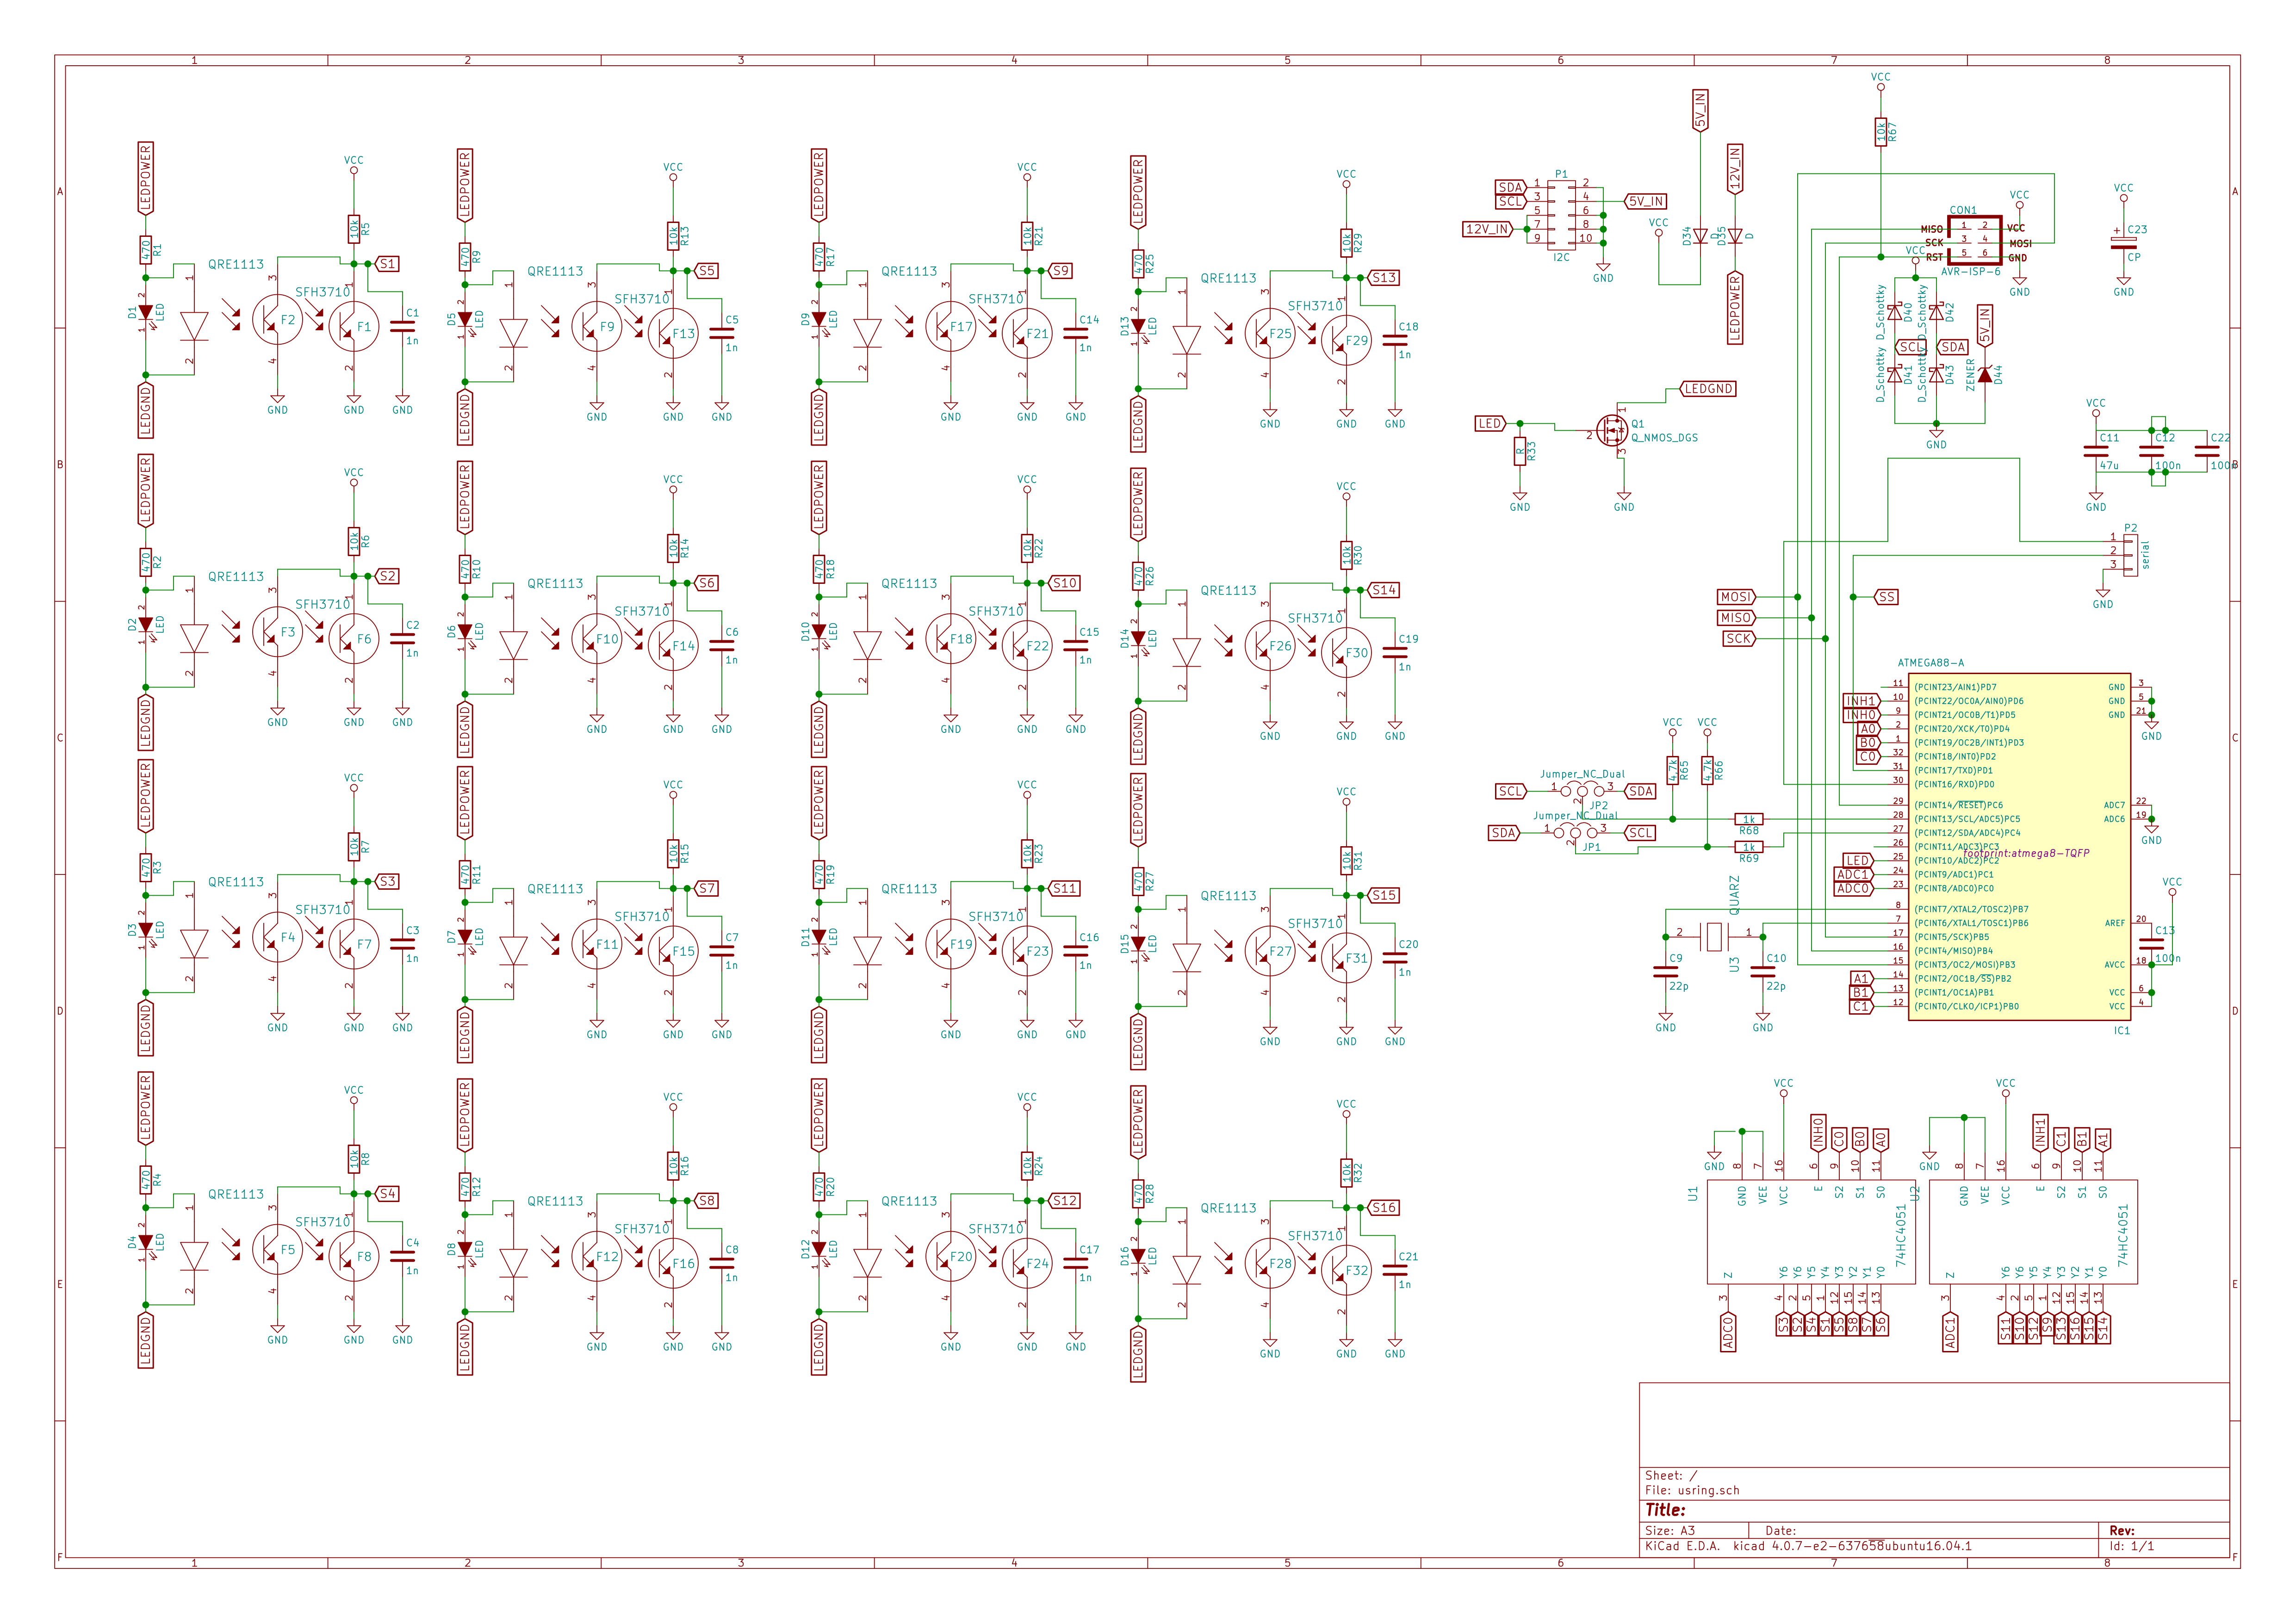
\includegraphics[height=10cm]{image/usring.jpg}
\subsection{Bemaßung}

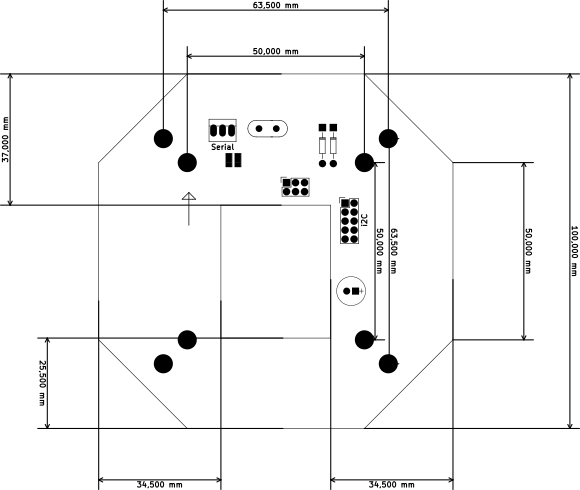
\includegraphics[height=10cm]{image/usring-dimensions.png}

%\subsection{Interface}




\section{Software}

\subsection{usring Klasse}


\begin{lstlisting}

class Usring{
	Usring();
	void getDifferenceValue(int* valueBuffer);
	uint8_t getAnalogValue(uint8_t id);
	void setLed(uint8_t state);
	void setI2C(uint8_t id, uint8_t value);
	void setI2CData(uint8_t id, uint8_t size, uint8_t* data);
	uint8_t getI2C(uint8_t id);
	void print(const char* string);
	void print(int value);
};

\end{lstlisting}

\subsection{Verwendung der usring Klasse}


\subsubsection{Konstruktor}

Initialisert die gesammte Hardware.
\begin{lstlisting}
Usring ring; // wie Goldboard gb;
\end{lstlisting}


\subsubsection{Sensor getDifferenceValue}
getDifferenceValue misst alle Sensoren einmal mit und einmal ohne LED Beleuchtung.
Die Differenz der Messung wird im int Array valueBuffer gespeichert. 
valueBuffer muss die Laenge 16 haben.
\begin{lstlisting}
ring.getDifferenceValue(int* valueBuffer);
\end{lstlisting}


\subsubsection{Sensor getAnalogValue}
getAnalogValue gibt den Analogwert des Sensors mit der Nummer id zurueck.
Achtung! Es wird keine Differenz gemessen.
\begin{lstlisting}
ring.getAnalogValue(uint8_t id);
\end{lstlisting}

\subsubsection{Sensor setLed}
setLed schaltet die LED an, wenn state > 0 und aus wenn state = 0 ist.
\begin{lstlisting}
ring.setLed(uint8_t state);
\end{lstlisting}


\subsubsection{I2C setI2C}
setI2C setzt den Wert value in das register mit der Nummer id.
Der Wert einer bestimmten id kann direkt ueber i2c vom Master ausgelesen werden.
\begin{lstlisting}
ring.setI2C(uint8_t id, uint8_t value);
\end{lstlisting}


\subsubsection{I2C setI2CData}
setI2CData setzt den Wert der Register mit der Nummer id bis zur Nummer id+size 
auf Werte in dem Array data mit der länge size.
\begin{lstlisting}
ring.setI2CData(uint8_t id, uint8_t size, uint8_t* data);
\end{lstlisting}
Beispiel:
\begin{lstlisting}
int x = 10; 
ring.setI2CData(0, 2, (uint8_t*)&x);
\end{lstlisting}


\subsubsection{I2C getI2C}
getI2C gibt den Wert des Eingangs Registers mit der Nummer id zurueck.
der I2C Master hat die Moeglichkeit diese Register zu setzen.
\begin{lstlisting}
ring.getI2C(uint8_t id);
\end{lstlisting}



\subsubsection{UART print}
gibt die Zeichenkette string ueber Uart aus.
\begin{lstlisting}
ring.print(const char* string);
\end{lstlisting}
gibt den Wert des Integeres value als ASCII ueber Uart aus.
\begin{lstlisting}
ring.print(int value);
\end{lstlisting}



\subsection{Beispielcode}


\begin{lstlisting}
#include "usring.h"

Usring ring;

int mittelwert[16];
int werte[16];
uint16_t ausgabe;

void kalibrieren()
{
	//mittelwerte auf 0 setzen
	for (int x = 0; x < 16; x++)
		mittelwert[x] = 0;
	
	//10 Messwerte Aufnehmen und den mittelwert Berechnen
	for (int x = 0; x < 10; x++)
	{
		ring.getDifferenceValue(werte);
		for (int i = 0; i < 16; i++)
			mittelwert[i] += werte[i];
		delay(10);
	}
	for (int x = 0; x < 16; x++)
		mittelwert[x] /= 10;
}

void messen()
{
	ring.getDifferenceValue(werte);
}

void berechnen()
{
	//Schwellwerte auswerten und 
	//    Ergebnisse in 16 bit Typ Speichern
	ausgabe = 0;
	for (int x = 0; x < 16; x++)
	{
		// offset auf den mittelwert addieren
		if (werte[x] > mittelwert[x] + 10) 	
		{
			// setze das bit auf 1 wenn der sensor was sieht
			ausgabe |= (1<<x); 
		}
	}
}


//daten in i2c Puffer Schreiben
void ausgeben()
{
	//16 bit Variable schreiben
	ring.setI2CData(0,2,(uint8_t*)&ausgabe); 
	for (int x = 0; x < 16; x++)
		//analog werte schreiben
		ring.setI2C(x+2, werte[x]); 
}

int main (void) {
	kalibrieren();
	while (1) {
		messen();
		berechnen();
		ausgeben();
	}                
}


\end{lstlisting}

\section{Bestellliste}

\begin{minipage}[t]{\textwidth}
	\begin{tabular}{llll}
		Package                             & Anzahl & Wert  &     \\
		R\_0805                             & 16       & 470R         &     \\
		R\_0805                             & 3        & 1k           &     \\
		R\_0805                             & 17       & 10k          &     \\
		R\_0805                             & 2        & 4,7k       &     \\
		C\_0805                             & 4        & 100n         &     \\
		C\_0805                             & 2        & 22p          &     \\
		CP\_Radial\_D8.0mm\_P2.50mm & 1        & 100u         &     \\
		SFH3710                             & 16       & SFH3710      &     \\
		1206\_LED                           & 16       & LED          &     \\
		Diode\_throughole                   & 2        & D            &     \\
		SMD-shotkey                         & 1        & ZENER 5,1V   &     \\
		SOT23                               & 1        & Q\_NMOS\_DGS &     \\
		QUARZ-HC49                          & 1        & QUARZ        &     \\
		Wannenstecker\_2x05                 & 1        & I2C          &     \\
		Shotkey-SOD-123                     & 4        & D\_Schottky  &     \\
		atmega8-TQFP                        & 1        & ATMEGA88-A   &     \\
		74HC4051-SO16                       & 2        & 74HC4051     &    
	\end{tabular}
\end{minipage}

\section{Bestückungsplan}

Bei der Bestückung ist zu beachten, dass der Pin VEE mit GND verbunden werden muss (neben dran)
die Verbindung mit VCC muss gekappt werden! Die Jumper 1 und 2 müssen wie folgt konfiguriert werden


\begin{minipage}[t]{\textwidth}
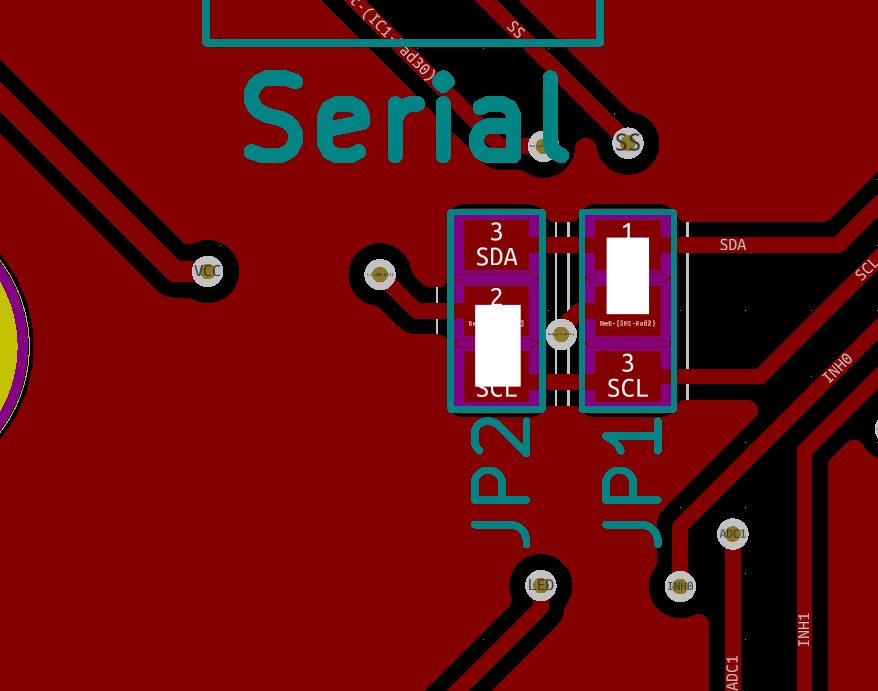
\includegraphics[height=5cm]{image/jumper.png}
\end{minipage}


\subsection{Oberseite}
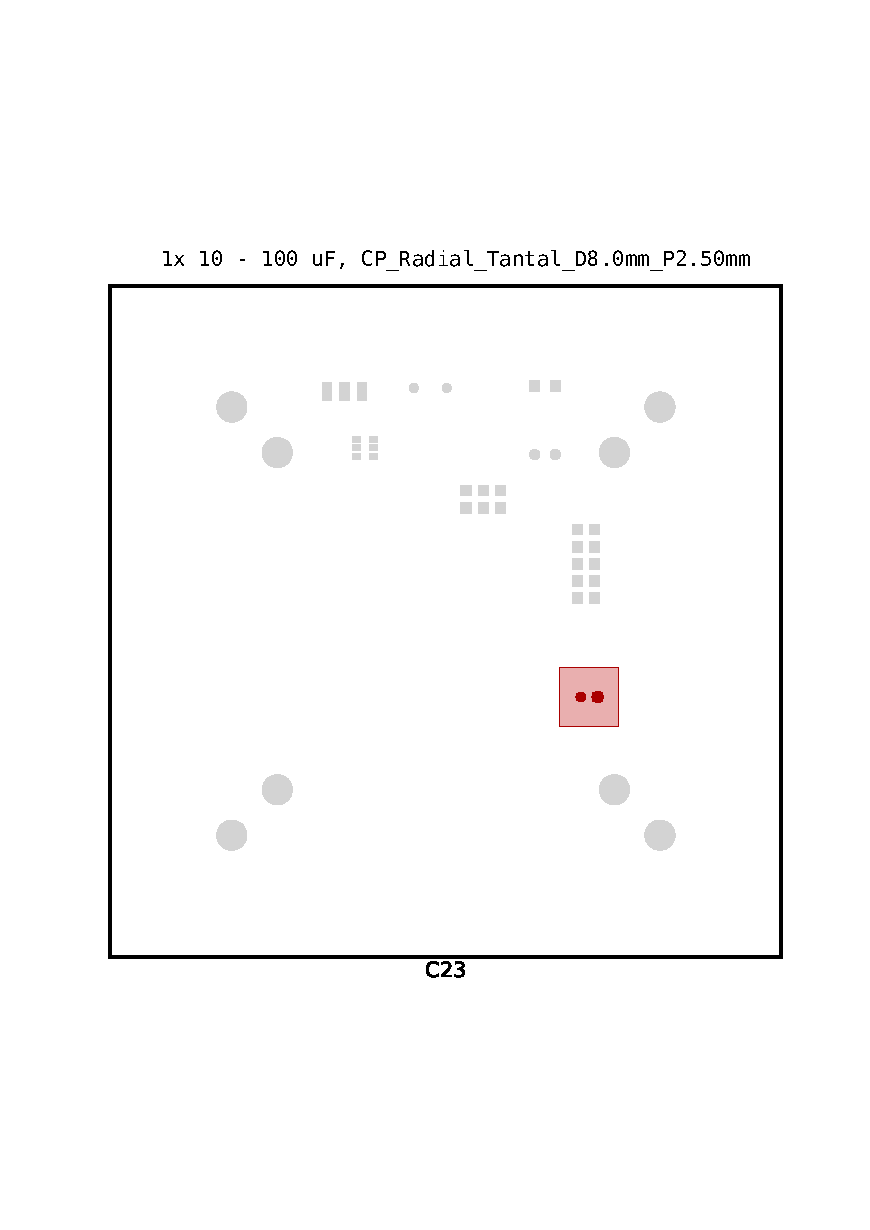
\includepdf[pages={1-5}]{image/usring_picknplace_TOP.pdf}

\subsection{Unterseite}
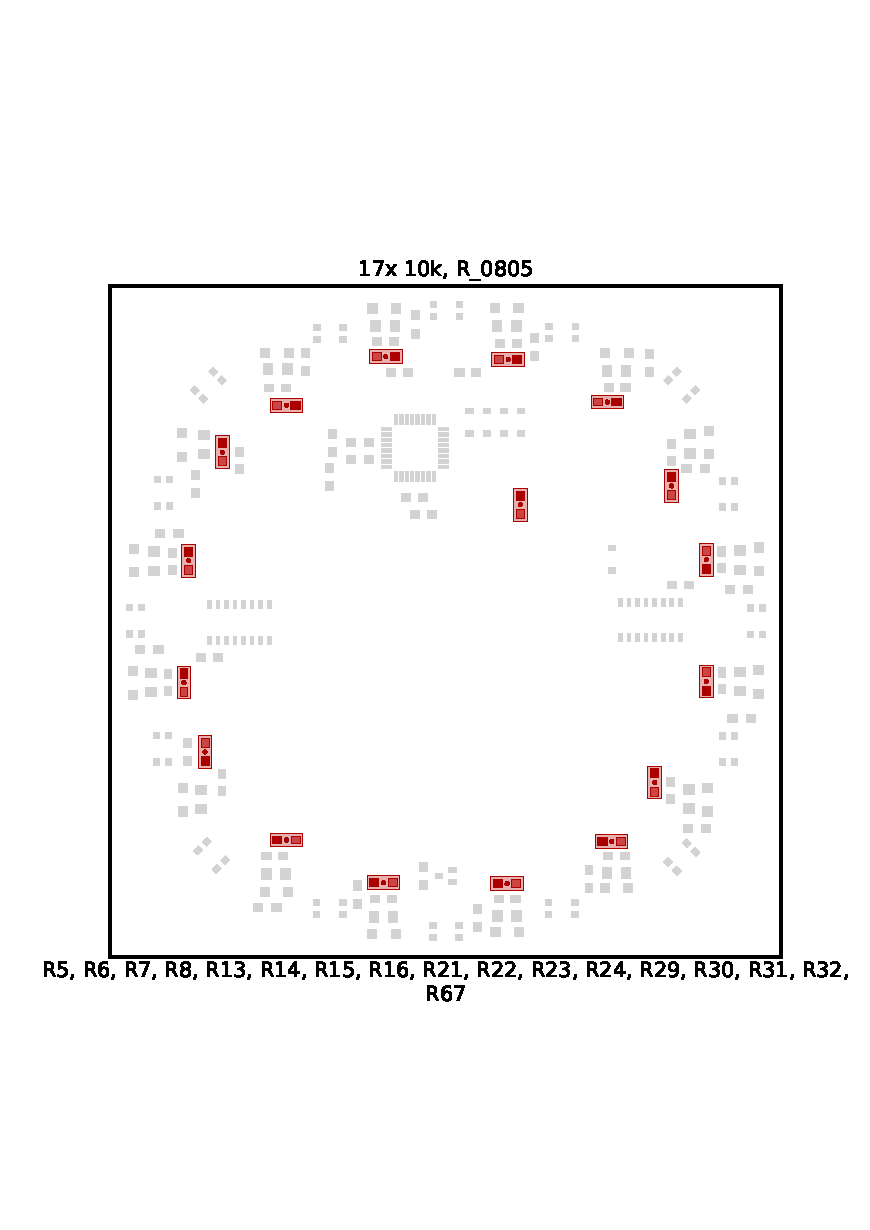
\includepdf[pages={1-13}]{image/usring_picknplace_BOTTOM.pdf}


\end{document}
